\chapter{Teorie modelů}\label{chapter:model-theory}

V této kapitole se trochu vzdálíme typickým aplikacím logiky v informatice\footnote{Například použití rezoluce k řešení otázky, zda v dané konečné teorii $T$ platí daná sentence $\varphi$.} a nahlédneme o úroveň abstrakce výše, do oblasti \emph{matematické} logiky. \emph{Teorie modelů} se snaží popsat vztah mezi obecnými vlastnostmi teorií (predikátové logiky) a tříd jejich modelů. Nevyhneme se práci s nekonečnými teoriemi a s nekonečnými strukturami. Jde jen o ukázku několika vybraných výsledků, které jsou pro nás dostupné. Ani se nepokusíme obsáhnout všechny hlavní oblasti teorie modelů, která je velmi bohatá a hluboká. Do této kapitoly jsme také přidali materiál týkající se vlastností modelů, který se nehodil jinam.


\section{Elementární ekvivalence}

Nejprve se podíváme na několik vlastností souvisejících s pojmem \emph{elementární ekvivalence}. Připomeňme, že $L$-struktury $\A$ a $\B$ jsou \emph{elementárně ekvivalentní} ($\A\equiv \B$), pokud v nich platí tytéž $L$-sentence.

V teorii modelů nás často zajímá, jaké vlastnosti (sentence) platí v dané, konkrétní struktuře:

\begin{definition}[Teorie struktury]
Mějme $L$-strukturu $\A$. \emph{Teorie struktury} $\A$, značíme $\Th(\A)$ je množina všech $L$-sentencí platných v $\A$:
$$
\Th(\A)=\{\varphi\mid\varphi\text{ je $L$-sentence a }\A\models\varphi\}
$$
\end{definition}

\begin{example}
Jako důležitý příklad vezměme \emph{standardní model aritmetiky}, strukturu $\underline{\mathbb{N}}=\langle\mathbb{N},S,+,\cdot,0,\le\rangle$. Teorii $\Th(\underline{\mathbb{N}})$ říkáme \emph{aritmetika přirozených čísel}. V následující kapitole si ukážeme, že je \emph{(algoritmicky) nerozhodnutelná}.\footnote{Teorie $T$ je \emph{(algoritmicky) rozhodnutelná}, pokud existuje algoritmus, který pro každou vstupní sentenci $\varphi$ doběhne a odpoví, zda $T\models\varphi$.}
\end{example}

Několik jednoduchých vlastností teorie struktury shrneme v následujícím pozorování:

\begin{observation}
    Nechť $\A$ je $L$-struktura a $T$ je $L$-teorie. Potom:
    \begin{enumerate}[(i)]
        \item Teorie $\Th(\A)$ je kompletní.
        \item Je-li $\A\in\M_L(T)$, potom $\Th(\A)$ je (kompletní) jednoduchá extenze teorie $T$.
        \item Pokud $\A\in\M_L(T)$ a $T$ je kompletní, potom je $\Th(\A)$ ekvivalentní s $T$, v tom případě $\Th(\A)=\Conseq_L(T)$.
    \end{enumerate}    
\end{observation}

Pomocí pojmu \emph{teorie struktury} můžeme také vyjádřit elementární ekvivalenci, pro $L$-struktury $\A,\B$ platí:
$$
\A\equiv\B \text{ právě když }\Th(\A)=\Th(\B).
$$

\begin{example}
   Podívejme se standardní uspořádání reálných, racionálních, a celých čísel, tj. na struktury $\langle\mathbb R,\leq\rangle$, $\langle\mathbb Q,\leq\rangle$, $\langle\mathbb Z,\leq\rangle$. Jak jsme již zmínili v Příkladu \ref{example:elementary-equivalence-of-orders-R-Q}, není těžké ukázat, že $\langle\mathbb R,\leq\rangle\equiv\langle\mathbb Q,\leq\rangle$ (pomocí \emph{hustoty} těchto uspořádání). Struktury $\langle\mathbb Q,\leq\rangle$ a $\langle\mathbb Z,\leq\rangle$ ale elementárně ekvivalentní nejsou: V $\langle\mathbb Z,\leq\rangle$ má každý prvek bezprostředního následníka, což v $\langle\mathbb Q,\leq\rangle$ neplatí. Pro následující sentenci $\varphi$ tedy máme $\varphi\in\Th(\langle\mathbb Z,\leq\rangle)$ ale $\varphi\not\in\Th(\langle\mathbb Q,\leq\rangle)$:
   $$
   \varphi=(\forall x)(\exists y)(x\leq y\land \neg x=y\land(\forall z)(x\leq z\limplies z=x\lor y\leq z))
   $$
\end{example}


\subsection{Kompletní jednoduché extenze}

Máme-li teorii $T$, zajímá nás, jak vypadají její modely. Připomeňme, že:
\begin{itemize}
    \item Teorie je \emph{kompletní}, právě když má jediný model až na elementární ekvivalenci.\footnote{Tedy všechny její modely jsou elementárně ekvivalentní.}
    \item Modely teorie $T$, až na elementární ekvivalenci, jednoznačně odpovídají kompletním jednoduchým extenzím $T$, až na ekvivalenci.
\end{itemize}
Kompletní jednoduché extenze $L$-teorie $T$ jsou tedy (až na ekvivalenci) tvaru $\Th(\A)$ pro $\A\in\M_L(T)$, a (jak jsme už zmínili výše) $\A\equiv\B$ právě když $\Th(\A)=\Th(\B)$. Místo hledání všech modelů tedy stačí najít všechny kompletní jednoduché extenze.

\begin{remark}
    Jednou z motivací, proč se zabývat kompletními jednoduchými extenzemi, je Tvrzení \ref{propositon:recursively-enumerable-completion} z následující kapitoly, které říká, že pokud lze \emph{efektivně (algoritmicky) popsat} všechny kompletní jednoduché extenze\footnote{Představte si algoritmus, který pro daná vstupní $i,j$ odpoví $j$-tý axiom $i$-té kompletní jednoduché extenze (v nějakém pevném očíslování); takový algoritmus ne vždy existuje!} \emph{efektivně dané} teorie $T$,\footnote{$T$ může být nekonečná, ale musí existovat algoritmus, který postupně vygeneruje všechny axiomy $T$.} potom je $T$ \emph{(algoritmicky) rozhodnutelná}.
\end{remark}


Schopnost (efektivně) popsat všechny kompletní jednoduché extenze je poměrně vzácná, a vyžaduje silné předpoklady. Přesto to lze provést u mnoha důležitých teorií. Uveďme jeden příklad: \emph{teorii hustého lineárního uspořádání (dense linear order)}.

\subsubsection{Příklad: DeLO*}

Teorie \emph{hustého lineárního uspořádání (DeLO*)}  je extenze teorie uspořádání o následující axiomy: 
\begin{itemize}
    \item axiom \emph{linearity} (někdy se mu říká také \emph{dichotomie}):
    $$
    x\leq y\lor y\leq x
    $$
    \item axiom \emph{hustoty}
    $$
    {x\leq y}\land{\neg\,x=y}\limplies(\exists z)(x\leq z\land z\leq y\land\neg\,z=x\land\neg\,z=y)
    $$
\end{itemize}
Někdy se přidává i axiom \emph{netriviality} $(\exists x)(\exists y)(\neg\,x=y)$ zakazující jednoprvkový model. Tato teorie není kompletní, umíme ale popsat všechny její kompletní jednoduché extenze:

\begin{proposition}
Mějme sentence $\varphi=(\exists x)(\forall y)(x\leq y)$ a $\psi=(\exists x)(\forall y)(y\leq x)$ vyjadřující existenci minimálního resp. maximálního prvku. Následující čtyři teorie jsou právě všechny (až na ekvivalenci) kompletní jednoduché extenze teorie DeLO*:
\begin{itemize}
    \item $\DeLO = \DeLO^*\ \cup \ \{\neg\varphi
    ,\neg\psi\}$
    \item $\DeLO^+ = \DeLO^*\ \cup \ \{\neg\varphi
    ,\psi\}$
    \item $\DeLO^- = \DeLO^*\ \cup \ \{\varphi
    ,\neg\psi\}$
    \item $\DeLO^\pm = \DeLO^*\ \cup \ \{\varphi
    ,\psi\}$        
\end{itemize}
\end{proposition}

Stačí ukázat, že tyto čtyři teorie jsou kompletní. Potom už je zřejmé, že žádná další kompletní jednoduchá extenze DeLO* nemůže existovat. Jak vysvětlíme v Sekci \ref{section:categoricity}, jejich kompletnost plyne z faktu, že jsou \emph{$\omega$-kategorické}, tj. mají jediný spočetný model až na \emph{izomorfismus}. Viz Důsledek \ref{corollary:complete-simple-extensions-of-delo}.


\subsection{Důsledky Löwenheim-Skolemovy věty}

V Sekci \ref{subsection:loewenheim-skolem-theorem} jsme dokázali tzv. Löwenheim-Skolemovu větu, konkrétně její variantu pro jazyky bez rovnosti:

\begin{theorem-unnumbered}[Löwenheim-Skolemova]
    Je-li $L$ spočetný jazyk bez rovnosti, potom každá bezesporná $L$-teorie má spočetně nekonečný model.
\end{theorem-unnumbered}

Tato věta má následující jednoduchý důsledek:

\begin{corollary}\label{corollary:loewenheim-skolem-without-equality}
    Je-li $L$ spočetný jazyk bez rovnosti, potom ke každé $L$-struktuře existuje elementárně ekvivalentní spočetně nekonečná struktura.
\end{corollary}
\begin{proof}
    Mějme $L$-strukturu $\A$. Teorie $\Th(\A)$ je bezesporná (má model $\A$), tedy dle Löwenheim-Skolemovy věty má spočetně nekonečný model $\B\models\Th(\A)$. To ale znamená, že $\B\equiv\A$.
\end{proof}
V jazyce bez rovnosti tedy nemůžeme vyjádřit například `model má právě 42 prvků'.

V důkazu Löwenheim-Skolemovy věty jsme sestrojený model získali jako kanonický model pro bezespornou větev tabla z $T$ pro položku $\F\bot$. Stejným způsobem se dokáže následující verze pro jazyky s rovností, stačí faktorizovat dle relace $=^A$:

\begin{theorem-unnumbered}[Löwenheim-Skolemova s rovností]
    Je-li $L$ spočetný jazyk s rovností, potom každá bezesporná $L$-teorie má spočetný model (tj. konečný, nebo spočetně nekonečný).
\end{theorem-unnumbered}

I tato verze má snadný důsledek pro konkrétní struktury:

\begin{corollary}\label{corollary:loewenheim-skolem-with-equality}
    Je-li $L$ spočetný jazyk s rovností, potom ke každé \emph{nekonečné} $L$-struktuře existuje elementárně ekvivalentní spočetně nekonečná struktura.
\end{corollary}
\begin{proof}
    Mějme nekonečnou $L$-strukturu $\A$. Stejně jako v důkazu Důsledku \ref{corollary:loewenheim-skolem-without-equality} (ale za použití Löwenheim-Skolemovy věty s rovností) najdeme spočetnou strukturu $\B\equiv\A$. Protože v $\A$ platí pro každé $n\in\mathbb N$ sentence vyjadřující `existuje alespoň $n$ prvků' (což lze pomocí rovnosti snadno zapsat), platí tato sentence i v $\B$, $\B$ tedy nemůže být konečná a musí být spočetně nekonečná.
\end{proof}

Tento důsledek použijeme, abychom ukázali, že existuje spočetné těleso, které je algebraicky uzavřené:  

\subsubsection*{Spočetné algebraicky uzavřené těleso}

Těleso $\A$ je \emph{algebraicky uzavřené}, pokud každý polynom nenulového stupně v něm má kořen. Těleso reálných čísel $\mathbb R$ není algebraicky uzavřené, neboť $x^2+1$ nemá v $\mathbb R$ kořen, stejně tak těleso $\mathbb Q$ (v něm nemá kořen ani $x^2-2$). Těleso komplexních čísel $\mathbb C$ algebraicky uzavřené je, je ale nespočetné.

Algebraickou uzavřenost lze vyjádřit pomocí následujících sentencí $\psi_n$, pro každé $n>0$:
$$
(\forall x_{n-1})\dots(\forall x_0)(\exists y)(y^n+x_{n-1}\cdot y^{n-1}+\dots+x_1\cdot y + x_0) = 0
$$
kde $y^k$ je zkratka za term $y\cdot y \cdot\ \cdots\ \cdot y$ (kde  $\cdot$ je aplikováno ($k-1$)-krát).

\begin{corollary}
    Existuje spočetné algebraicky uzavřené těleso.
\end{corollary}
\begin{proof}
    Dle Důsledku \ref{corollary:loewenheim-skolem-with-equality} existuje spočetně nekonečná struktura $\A$ elementárně ekvivalentní tělesu $\mathbb C$. Protože $\mathbb C$ je těleso a splňuje sentence $\psi_n$ pro všechna $n>0$, je i $\A$ algebraicky uzavřené těleso.
\end{proof}


\section{Izomorfismus struktur}\label{section:isomorphism-of-structures}

Podívejme se blíže na pojem \emph{izomorfismu struktur}, který zobecňuje izomorfismus grafů, vektorových prostorů, apod. Neformálně řečeno, struktury jsou \emph{izomorfní}, pokud se liší jen pojmenováním konkrétních prvků.

\begin{definition}
Mějme struktury $\A,\B$ jazyka $L=\langle\mathcal R,\mathcal F\rangle$. \emph{Izomorfismus $\A$ a $\B$} (nebo `$\A$ \emph{na} $\B$') je bijekce $h\colon A\to B$ splňující následující vlastnosti:
\begin{itemize}
    \item Pro každý ($n$-ární) funkční symbol $f\in\mathcal F$ a pro všechna $a_i\in A$ platí:
    $$
    h(f^\A(a_1,\dots,a_n))=f^\B(h(a_1),\dots,h(a_n))
    $$
    (Speciálně, je-li $c\in\mathcal F$ konstantní symbol, platí $h(c^\A)=c^\B$.)
    \item Pro každý ($n$-ární) relační symbol $R\in\mathcal R$ a pro všechna $a_i\in A$ platí:
    $$
    R^\A(a_1,\dots,a_n)\ \text{ právě když }\ R^\B(h(a_1),\dots,h(a_n))
    $$
\end{itemize}
Pokud existuje, říkáme, že $\A$ a $\B$ jsou \emph{izomorfní} (nebo `$\A$ je \emph{izomorfní s $\B$ via $h$}') a píšeme $\A\simeq\B$ (nebo $\A\simeq_h\B$). \emph{Automorfismus} $\A$ je izomorfismus $\A$ na $\A$.
\end{definition}

Všimněte si, že relace `býti izomorfní' je ekvivalence. Ukažme si jeden příklad:

\begin{example}
    Je-li $|X|=n$, je potenční algebra $\underline{\mathcal P(X)}=\langle \mathcal P(X),-,\cap,\cup,\emptyset,X\rangle$ izomorfní s Booleovou algebrou  $\underline{2^n}=\langle \{0,1\}^n,-_n,\land_n,\lor_n,(0,\dots,0),(1,\dots,1)\rangle$ (kde operace aplikujeme po složkách) via $h(A)=\chi_A$, kde $\chi_A$ je charakteristický vektor podmnožiny $A\subseteq X$.
\end{example}

Nyní ukážeme, že izomorfismus je bijekce `zachovávající sémantiku':

\begin{proposition}
Mějme struktury $\A,\B$ jazyka $L=\langle\mathcal R,\mathcal F\rangle$. Bijekce $h\colon A\to B$ je izomorfismus $\A$ a $\B$, právě když platí následující:
\begin{enumerate}[(i)]
    \item pro každý $L$-term $t$ a ohodnocení proměnných $e:\Var\to A$:
    $$
    h(t^\A[e])=t^\B[e\circ h]
    $$
    \item pro každou $L$-formuli $\varphi$ a ohodnocení proměnných $e:\Var\to A$:
    $$
    \A\models \varphi[e]\ \text{ právě když }\ \B\models\varphi[e\circ h]
    $$
\end{enumerate}
\end{proposition}
\begin{proof}
    Je-li $h$ izomorfismus, vlastnosti snadno dokážeme indukcí podle struktury termu resp. formule. Naopak, je-li $h$ bijekce splňující (i) a (ii), dosazením $t=f(x_1,\dots,x_n)$ resp. $\varphi=R(x_1,\dots,x_n)$ dostáváme vlastnosti z definice izomorfismu.
\end{proof}

Jako okamžitý důsledek dostáváme fakt, že izomorfní struktury jsou elementárně ekvivalentní:

\begin{corollary}\label{corollary:isomorphic-implies-elementarily-equivalent}
    Pokud $\A\simeq\B$, potom $\A\equiv\B$.
\end{corollary}

\begin{remark}
    Obrácená implikace ale obecně neplatí, například pro uspořádané množiny racionálních a reálných čísel platí $\langle\mathbb Q,\leq \rangle\equiv\langle\mathbb R,\leq\rangle$ ale $\langle\mathbb Q,\leq \rangle\not\simeq \langle \mathbb R,\leq\rangle$ neboť $\mathbb Q$ je spočetná množina zatímco $\mathbb R$ není (neexistuje tedy mezi nimi žádná bijekce).
\end{remark}

Pro konečné modely ale platí, že izomorfismus je totéž co elementární ekvivalence, máme-li jazyk s rovností, jak dokážeme v následujícím tvrzení:

\begin{proposition}
    Je-li $L$ jazyk s rovností a $\A,\B$ konečné $L$-struktury, potom platí:
    $$
    \A\simeq\B\ \text{ právě když }\ \A\equiv\B
    $$
\end{proposition}
\begin{proof}
    Jednu implikaci jsme dokázali v Důsledku \ref{corollary:isomorphic-implies-elementarily-equivalent}. Předpokládejme, že $\A\equiv\B$ a ukažme, že existuje izomorfismus $\A$ na $\B$. Protože je jazyk s rovností, můžeme vyjádřit sentencí, že `existuje právě $n$ prvků'. Z toho plyne, že $|A|=|B|$.

    Označme jako $\A'$ expanzi $\A$ o jména prvků z $A$; jde o strukturu v jazyce $L'=L\cup\{c_a\mid a\in A\}$. Ukážeme, že $\B$ lze expandovat na $L'$-strukturu $\B$ tak, že $\A'\equiv \B'$. Potom, jak lze snadno ověřit, je zobrazení $h(a)= c_a^{\B'}$ izomorfismem $\A'$ na $\B'$, a tedy i izomorfismem jejich $L$-reduktů a $\A\simeq\B$.

    Stačí ukázat, že pro každé $c_a^{\A'}=a\in A$ existuje prvek $b\in B$ takový, že pro expanze o interpretaci konstantního symbolu $c_a$ platí $\langle  \A,a\rangle\equiv\langle\B,b\rangle$. Označme jako $\Omega$ množinu formulí $\varphi(x)$ takových, že $\langle \A,a\rangle \models \varphi(x/c_a)$, neboli $\A\models \varphi[e(x/a)]$. Protože je $A$ konečná množina, existuje konečně mnoho formulí $\varphi_1(x),\dots,\varphi_m(x)$ takových, že pro každou formuli $\varphi \in \Omega$ existuje $i$ takové, že $\A\models \varphi\liff\varphi_i$. Potom i $\B\models\varphi\liff\varphi_i$ (neboť $\A\equiv\B$, stačí vzít generální uzávěr této formule, což je sentence).
    
    Protože v $\A$ platí sentence $(\exists x)\bigwedge_{i=1}^m\varphi_i$ (je splněna díky prvku $a\in A$) a $\B\equiv\A$, máme i $\B\models (\exists x)\bigwedge_{i=1}^m\varphi_i$. Jinými slovy, existuje $b\in B$ takové, že $\B\models\bigwedge_{i=1}^m\varphi_i[e(x/b)]$. Tedy pro každou $\varphi\in \Omega$ platí $\B\models \varphi[e(x/b)]$, tj. $\langle\mathcal{B},b\rangle\models \varphi(x/c_a)$, což jsme chtěli dokázat.
\end{proof}

\begin{corollary}
    Pokud má kompletní teorie v jazyce s rovností konečný model, potom jsou všechny její modely izomorfní.
\end{corollary}


\subsection{Definovatelnost a automorfismy}

Připomeňme si pojem definovatelné množiny, viz Sekce \ref{section:definability}. Ukážeme si užitečnou vlastnost definovatelných množin: jsou uzavřené (`invariantní') na automorfismy dané struktury. 

Nikoho nepřekvapí, že při automorfismu se musí izolovaný vrchol daného grafu zobrazit na izolovaný vrchol, vrchol stupně 4 na vrchol stejného stupně, nebo třeba trojice vrcholů, která tvoří trojúhelník, na trojúhelník. To nám může pomoci například při hledání automorfismů.

\begin{proposition}
    Je-li $D\subseteq A^n$ definovatelná ve struktuře $\A$, potom pro každý automorfismus $h\in\Aut(\A)$ platí $h[D]=D$ (kde $h[D]$ značí $\{h(\overline{a})\mid\overline{a}\in D\}$).

    Je-li $D$ definovatelná s parametry $\overline{b}$, platí totéž pro automorfismy identické na $\overline{b}$ (\emph{fixující} $\overline{b}$), tj. takové, že $h(\overline{b})=\overline{b}$ (neboli $h(b_i)=b_i$ pro všechna $i$).
\end{proposition}
\begin{proof}
    Ukážeme jen verzi s parametry. Nechť $D=\varphi^{\A,\overline{b}}(\overline{x},\overline{y})$. Potom pro každé $\overline{a}\in A^n$ platí následující ekvivalence:
\begin{align*}
\overline{a}\in D\ 
&\Leftrightarrow\ \A\models \varphi[e(\overline{x}/\overline{a},\overline{y}/\overline{b})]\\
&\Leftrightarrow\  \A\models \varphi[(e\circ h)(\overline{x}/\overline{a},\overline{y}/\overline{b})]\\
&\Leftrightarrow\ \A\models \varphi[e(\overline{x}/h(\overline{a}),\overline{y}/h(\overline{b}))]\\
&\Leftrightarrow\ \A\models \varphi[e(\overline{x}/h(\overline{a}),\overline{y}/\overline{b})]\\
&\Leftrightarrow\ h(\overline{a})\in D.
\end{align*}
\end{proof}

\begin{example}
    Uvažme následující graf $\mathcal G$. Najděme všechny množiny definovatelné z $\mathcal G$ s parametrem $0$, tj. množinu 
    $\mathrm{Df}^1(\mathcal G,\{0\})$. 
    \begin{center}
        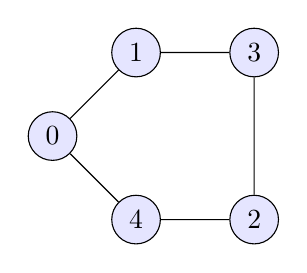
\begin{tikzpicture}[every node/.style={circle,fill=blue!10,draw,minimum size=0.5cm,node distance=1.5cm}]
            \node (1) {$1$};
            \node[below left of=1](0) {$0$};
            \node[below right of=0] (4) {$4$};
            \node[right of=4] (3) {$2$};
            \node[right of=1] (2) {$3$};
            \path[draw] (0) -- (1) -- (2) -- (3) -- (4) -- (0);
        \end{tikzpicture}
    \end{center}
    Tento graf má jediný netriviální automorfismus zachovávající vrchol $0$: $h(i)=(5-i) \bmod 5$. Jeho \emph{orbity} jsou $\{0\}$, $\{1,4\}$, a $\{2,3\}$. Tyto množiny jsou definovatelné:
    \begin{itemize}
        \item $\{0\}$ je definované formulí $x=y$, tj. $(x=y)^{\mathcal G,\{0\}}=\{0\}$,
        \item $\{1,4\}$ lze definovat pomocí formule $E(x,y)$, a
        \item $\{2,3\}$ formulí $\neg E(x,y)\land \neg x=y$.
    \end{itemize}
    Množina $\mathrm{Df}^1(\mathcal G,\{0\})$ je podalgebra potenční algebry $\underline{\mathcal P(V(\mathcal G))}$, musí tedy být uzavřená na doplněk, sjednocení, průnik, a obsahovat $\emptyset$ a $V(\mathcal G)$. Podalgebra generovaná $\{\{0\},\{1,4\},\{2,3\}\}$ už ale obsahuje všechny podmnožiny zachovávající automorfismus $h$. Dostáváme:
    $$
    \mathrm{Df}^1(\mathcal G,\{0\})=\{\emptyset, \{0\}, \{1,4\}, \{2,3\}, \{0,1,4\}, \{0,2,3\}, \{1,4,2,3\}, \{0,1,2,3,4\}\}
    $$
\end{example}

\begin{exercise}
    Uvažme následující graf. Najděte všechny automorfismy. Určete, které podmnožiny jsou definovatelné, uveďte definující formule. Které binární relace jsou definovatelné?
    \begin{center}
        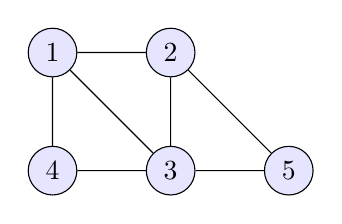
\begin{tikzpicture}[every node/.style={circle,fill=blue!10,draw,minimum size=0.5cm,node distance=1.5cm}]
            \node (1) {$1$};
            \node[right of=1] (2) {$2$};
            \node[below of=2] (3) {$3$};
            \node[left of=3] (4) {$4$};
            \path[draw] (1) -- (2) -- (3) -- (4) -- (1) -- (3);
            \node[right of=3] (5) {$5$};
            \path[draw] (2) -- (5) -- (3);
        \end{tikzpicture}
    \end{center}
\end{exercise}


\section{$\omega$-kategorické teorie}\label{section:categoricity}

Nyní se podíváme na teorie, které mají jediný spočetně nekonečný model (až na izomorfismus), říkáme jim \emph{$\omega$-kategorické}.\footnote{Symbol $\omega$ se používá pro nejmenší nekonečné \emph{ordinální} číslo, jinými slovy, pro množinu všech přirozených čísel.}

\begin{definition}[Izomorfní spektrum, $\kappa$-kategoricita]
    \emph{Izomorfní spektrum} teorie $T$ je počet $
    I(\kappa,T)$ modelů $T$ kardinality $\kappa$ až na izomorfismus, pro každou kardinalitu $\kappa$ (včetně \emph{transfinitních}).     Teorie $T$ je \emph{$\kappa$-kategorická}, pokud $
    I(\kappa,T)=1$.
\end{definition}

Nadále nás bude zajímat jen případ $\kappa=\omega$, totiž teorie s jediným spočetně nekonečným modelem (až na izomorfismus). Jako příklad uveďme teorii hustého lineárního uspořádání bez konců:

\begin{proposition}
    Teorie DeLO je $\omega$-kategorická.
\end{proposition}
\begin{proof}
Vezměme dva spočetně nekonečné modely $\A,\B$ a očíslujme jejich prvky: $A=\{a_i\mid i\in\mathbb N\}$, $B=\{b_i\mid i\in\mathbb N\}$. Indukcí podle $n$ lze díky hustotě nalézt posloupnost $h_0\subseteq h_1\subseteq h_2\subseteq\dots$ prostých (parciálních) funkcí z $A$ do $B$, takových, že $\{a_0,\dots,a_{n-1}\}\subseteq\dom h_n$, $\{b_0,\dots,b_{n-1}\}\subseteq\rng h_n$,\footnote{Zde $\dom$ značí \emph{doménu} a $\rng$ značí \emph{obor hodnot (`range')} funkce.} a \emph{zachovávají uspořádání}\footnote{Tj. je-li $a_i,a_j\in\dom h_n$, potom $a_i\leq^\A a_j$ právě když $h(a_i)\leq^\B h(a_j)$.} Potom $\A\simeq\B$ via $h=\bigcup_{n\in\mathbb N}h_n$.
\end{proof}

\begin{corollary}
Izomorfní spektrum teorie DeLO* je následující:
$$
I(\kappa,DeLO^*)=\begin{cases}
    0 &\text{pro }\kappa\in\mathbb{N},\\
    4 &\text{pro }\kappa=\omega.
\end{cases}
$$
Spočetné modely až na izomorfismus jsou například:
$$ 
\mathbb Q=\langle \mathbb Q,\leq\rangle\simeq\mathbb Q\upharpoonright(0,1), \ \mathbb Q\upharpoonright(0,1], \ \mathbb Q \upharpoonright [0,1), \ \mathbb Q \upharpoonright [0,1]
$$
\end{corollary}

\begin{proof}
Husté uspořádání jistě nemůže být konečné. Izomorfismus musí zobrazit nejmenší prvek na nejmenší prvek, a největší na největší.
\end{proof}

Pojem \emph{$\omega$-kategoricity} lze chápat jako zeslabení pojmu \emph{kompletnosti}. Platí následující užitečné kritérium:

\begin{theorem}[$\omega$-kategorické kritérium kompletnosti]
Mějme $\omega$-kategorickou teorii $T$ ve spočetném jazyce $L$. Je-li
\begin{itemize}
    \item $L$ bez rovnosti, nebo
    \item $L$ s rovností a $T$ nemá konečné modely,
\end{itemize}
potom je teorie $T$ kompletní.
\end{theorem}
\begin{proof}
Pro jazyk bez rovnosti víme z Důsledku \ref{corollary:loewenheim-skolem-without-equality} Löwenheim-Skolemovy věty, že každý model je elementárně ekvivalentní nějakému spočetně nekonečnému modelu. Ten je ale až na izomorfismus jediný, takže všechny modely jsou elementárně ekvivalentní, což je sémantická definice kompletnosti.

Máme-li jazyk s rovností, použijeme podobně Důsledek \ref{corollary:loewenheim-skolem-with-equality} a dostaneme, že všechny nekonečné modely jsou elementárně ekvivalentní. Mohly by existovat elementárně neekvivalentní konečné modely, to jsme ale zakázali.
\end{proof}

\begin{corollary}\label{corollary:complete-simple-extensions-of-delo}
    Teorie $\DeLO$, $\DeLO^+$, $\DeLO^-$, a $\DeLO^\pm$ jsou kompletní. Jsou to všechny (navzájem neekvivalentní) kompletní jednoduché extenze teorie $DeLO^*$.
\end{corollary}

\begin{remark}
Analogické kritérium platí i pro kardinality $\kappa$ větší než $\omega$.
\end{remark}


\section{Axiomatizovatelnost}\label{section:axiomatizability}

Na závěr této kapitoly se podíváme, za jakých okolností lze `popsat' (\emph{axiomatizovat}) třídu modelů respektive teorii. Zajímat nás bude také kdy si vystačíme s konečně mnoha axiomy, a kdy to lze pomocí otevřených axiomů (kterých může být i nekonečně mnoho). Srovnejte s Tvrzením \ref{proposition:axiomatize-in-DNF-CNF} z výrokové logiky. 

\begin{definition}[Axiomatizovatelnost]
Mějme třídu struktur $K\subseteq\M_L$ v nějakém jazyce $L$. Říkáme, že $K$ je
\begin{itemize}
    \item \emph{axiomatizovatelná}, pokud existuje $L$-teorie $T$ taková, že $\M_L(T)=K$,
    \item \emph{konečně axiomatizovatelná}, pokud je axiomatizovatelná konečnou teorií, a
    \item \emph{otevřeně axiomatizovatelná}, pokud je axiomatizovatelná otevřenou teorií.
\end{itemize}
O $L$-teorii $T'$ říkáme, že je \emph{konečně} resp. \emph{otevřeně axiomatizovatelná}, pokud to platí o třídě modelů $K=\M_L(T')$.
\end{definition}

\begin{example}
    Uveďme několik příkladů:
    \begin{itemize}
        \item grafy nebo částečná uspořádání jsou konečně i otevřeně axiomatizovatelné,
        \item tělesa jsou konečně, ale ne otevřeně axiomatizovatelná,
        \item nekonečné grupy jsou axiomatizovatelné, ale ne konečně axiomatizovatelné,
        \item konečné grafy nejsou axiomatizovatelné.
    \end{itemize}
    Proč tomu tak je ukážeme níže.
\end{example}

Začněme jednoduchým faktem:

\begin{observation}
    Je-li $K$ axiomatizovatelná, musí být uzavřená na elementární ekvivalenci.  
\end{observation}

Z věty o kompaktnosti snadno získáme následující tvrzení, pomocí kterého lze ukázat neaxiomatizovatelnost např. konečných grafů, konečných grup, konečných těles.

\begin{theorem}
    Pokud má teorie libovolně velké konečné modely, potom má i nekonečný model. V tom případě není třída všech jejích konečných modelů axiomatizovatelná.
\end{theorem}
\begin{proof}
    Je-li jazyk bez rovnosti, stačí vzít kanonický model pro některou bezespornou větev v tablu z $T$ pro položku $\F\bot$ ($T$ je bezesporná, neboť má model(y), tedy tablo není sporné).     
    
    Mějme jazyk s rovností a označme jako $T'$ následující extenzi teorie $T$ do jazyka rozšířeného o spočetně mnoho nových konstantních symbolů $c_i$:
    $$
    T'=T \cup \{\neg c_i = c_j \mid i\neq j\in\mathbb N\}
    $$
    Každá konečná část teorie $T'$ má model: nechť $k$ je největší takové, že symbol $c_k$ se vyskytuje v této konečné části $T'$. Potom stačí vzít libovolný alespoň $(k+1)$-prvkový model $T$ a interpretovat konstanty $c_0,\dots,c_k$ jako navzájem různé prvky tohoto modelu.

    Dle věty o kompaktnosti má potom i $T'$ model. Ten je nutně nekonečný. Jeho redukt na původní jazyk (zapomenutí konstant $c_i^\A$) je nekonečným modelem $T$.
\end{proof}

\begin{remark}
    Třída všech \emph{nekonečných} modelů teorie ale je vždy axiomatizovatelná, máme-li jazyk s rovností: stačí k teorii přidat pro každé $n\in\mathbb N$ axiom vyjadřující `existuje alespoň $n$ prvků'.
\end{remark}


\subsection{Konečná axiomatizovatelnost}

Ukážeme následující kritérium konečné axiomatizovatelnosti: jak třída struktur $K$ tak i $\overline{K}$ musí být axiomatizovatelné.

\begin{theorem}[O konečné axiomatizovatelnosti]\label{theorem:finite-axiomatizability}
    Mějme třídu struktur $K\subseteq \M_L$ a uvažme také její doplněk $\overline{K}=\M_L\setminus K$. Potom $K$ je konečně axiomatizovatelná, právě když $K$ i $\overline{K}$ jsou axiomatizovatelné.   
\end{theorem}
\begin{proof}
Je-li $K$ konečně axiomatizovatelná, potom je axiomatizovatelná i konečně mnoha sentencemi $\varphi_1,\dots,\varphi_n$ (nahradíme formule jejich generálními uzávěry). Jako axiomatizaci $\overline{K}$ stačí vzít sentenci $\psi=\neg(\varphi_1\land\varphi_2\land\dots\land\varphi_n)$. Zřejmě platí $\M(\psi)=\overline{K}$.

Naopak, nechť $T$ a $S$ jsou teorie takové, že $\M(T)=K$ a $\M(S)=\overline{K}$. Uvažme teorii $T\cup S$. Tato teorie je sporná, neboť:
$$
\M(T\cup S)=\M(T)\cap \M(S)=K\cap\overline{K}=\emptyset
$$
Podle věty o kompaktnosti\footnote{Vidíte, jak je užitečná!} existují konečné podteorie $T'\subseteq T$ a $S'\subseteq S$ takové, že:
$$
\emptyset = \M(T'\cup S')=\M(T')\cap \M(S')
$$
Nyní si všimněme, že platí
$$
\M(T)\subseteq \M(T')\subseteq \overline{\M(S')}\subseteq \overline{\M(S)}=\M(T)
$$
tím jsme dokázali, že $M(T)=M(T')$, tj. teorie $T'$ je hledanou konečnou axiomatizací $K$.
\end{proof}

Jako aplikaci si dokážeme, že tělesa charakteristiky 0 nejsou konečně axiomatizovatelná.

\subsubsection*{Příklad: tělesa charakteristiky 0}
 
Nechť $T$ je teorie těles. Charakteristika tělesa je nejmenší počet jedniček, které je třeba sečíst, abychom dostali nulu (v tom případě musí být charakteristika prvočíslo---dokažte si!), nebo, pokud nikdy nedostaneme sčítáním jedniček nulu, říkáme že je charakteristika 0. Trochu formálněji:

\begin{definition}[Charakteristika tělesa]
Říkáme, že těleso $\A=\langle A,+,-,0,\cdot,1 \rangle$ je
\begin{itemize}
    \item \emph{charakteristiky $p$}, je-li $p$ nejmenší prvočíslo takové, že $\A\models p1=0$, kde $p1$ označuje term $1+1+\dots+1$ s $p$ jedničkami, nebo
    \item \emph{charakteristiky 0}, pokud není charakteristiky $p$ pro žádné prvočíslo $p$.
\end{itemize}
\end{definition}
Nechť $T$ je teorie těles. Potom třída těles charakteristiky $p$ je konečně axiomatizována teorií $T\cup \{p1=0\}$. Třída těles charakteristiky 0 je axiomatizována následující (nekonečnou) teorií:
$$
T'=T\cup \{\neg\, p1=0\mid p\text{ je prvočíslo}\}
$$
Konečná axiomatizace ale neexistuje.

\begin{proposition}
Třída $K$ těles charakteristiky $0$ není konečně axiomatizovatelná.   
\end{proposition}
\begin{proof}
Díky Větě \ref{theorem:finite-axiomatizability} stačí ukázat, že $\overline{K}$ (sestávající z těles nenulové charakteristiky a struktur, které nejsou tělesa) není axiomatizovatelná, což dokážeme sporem. Nechť existuje teorie $S$ taková, že $\M(S)=\overline{K}$. Potom teorie 
$S'=S\cup T'$ má model, neboť každá její konečná část má model: stačí vzít těleso prvočíselné charakteristiky větší než jakékoliv $p$ z axiomu $T'$ tvaru $\neg\, p1=0$. Nechť $\A$ je model $S'$. Potom je i $\A\in\M(S)=\overline{K}$. Zároveň je ale $\A\in\M(T')=K$, což je spor.
\end{proof}

\subsection{Otevřená axiomatizovatelnost}

Pro otevřenou axiomatizovatelnost existuje jednoduché sémantické kritérium: třída jejích modelů musí být uzavřená na podstruktury. Platí dokonce ekvivalence, dokážeme ale jen jednu implikaci (důkaz druhé je obtížnější).

\begin{theorem}\label{theorem:open-axiomatizability}
Pokud je teorie $T$ otevřeně axiomatizovatelná, potom je každá podstruktura modelu $T$ také modelem $T$.   
\end{theorem}

\begin{remark}
    Platí i obrácená implikace: Je-li každá podstruktura modelu $T$ také modelem, potom je $T$ otevřeně axiomatizovatelná. Důkaz zde ale neuvedeme.
\end{remark}

\begin{proof}
Nechť $T'$ je otevřená axiomatizace $T$. Mějme model $\A\models T'$  a podstrukturu $\B\subseteq\A$. Pro každou formuli $\varphi\in T'$ platí $\B\models\varphi$ (neboť $\varphi$ je otevřená), tedy i $\B\models T'$.  
\end{proof}

\begin{example}
    Uveďme několik příkladů:
    \begin{itemize}
        \item Teorie DeLO není otevřeně axiomatizovatelná, například žádná konečná podstruktura modelu DeLO nemůže být hustá.
        \item Teorie těles není otevřeně axiomatizovatelná, podstruktura $\mathbb Z\subseteq\mathbb Q$ tělesa racionálních čísel není tělesem, v $\mathbb Z$ neexistuje inverzní prvek vůči násobení k číslu $2$.
        \item Pro dané $n\in\mathbb N$ jsou nejvýše $n$-prvkové grupy otevřeně axiomatizovatelné(podgrupy jsou jistě také nejvýše $n$-prvkové). Jako otevřenou axiomatizaci lze vzít následující extenzi (otevřené) teorie grup $T$:
        $$
        T\cup \{\bigvee_{1\leq i<j\leq n+1}x_i=x_j\}
        $$
    \end{itemize}
\end{example}
